%!TEX root = ../thesis.tex
%*******************************************************************************
%*********************************** Eight Chapter *****************************
%*******************************************************************************

\chapter{General conclusion and future work}  %Title of the First Chapter

\ifpdf
    \graphicspath{{Chapter11/Figs/Raster/}{Chapter11/Figs/PDF/}{Chapter11/Figs/}}
\else
    \graphicspath{{Chapter11/Figs/Vector/}{Chapter11/Figs/}}
\fi

One of the main aims of this thesis has been accomplished. The design of a bioelectrical impedance plethysmographic device capable of taking measurements in a home setting. The device created has the potential to operate using batteries as a Class II device. The device has the capability of being portable. However, the design can be further miniaturised to improve its transportability.  During the experimental procedure was demonstrated the performance of the device. It is clear that with the instrument is possible to perform tests doing VOP or just analysis of the arterial pulses. The output channels provide the necessary data to calculate the impedance in a section of the body measuring the current being delivered, the potential of the basal impedance and the arterial pulses of the AC component. 

The design of the instrument also included software that helped to clean up the signal and fast processing the waveforms. At present, it is only possible to perform off-line measurements. But it the near future, with the algorithms implemented it would be possible to measure beat by beat, changes of volume or quantifying blood flow.

The other aims of the thesis were focused on the analysis of the waveforms and its correlation to other instruments.  As it was shown, all the devices used in the experiment provided data synchronised to the systolic peak. The following sections will give a further critique of the findings from the analysis of these signals. 


%********************************** %First Section  **************************************
\section{Converting iPG into Blood Flow for detecting venous and arterial changes} %Section - 7.1 
\label{section discussion 1}
As it has been discussed in this document, there are two ways to calculate blood flow from the iPG data. Initially, it is needed to model the segment of the body as a cylinder. Luckily, this geometrical form is common in most parts of the body. For this study, a device was designed to measure the change of volume in the forearm. Eventually, this could be calibrated to work in other parts of the body such as lower extremities. 

The study performed in this document seeks to demonstrate how the iPG data could help to detect changes in venous and arterial circulation. According to the literature, iPG is a method used to quantify blood flow from the principle that the impedance of a body part is directly proportional to its volume as described by Nyober's equation  (see equation \ref{eq:nyober dV}).  Hence, since the 1970's this theory has been tested assuring the effectiveness of the method. 

There are different contributors to the impedimetric signal. One of them is the tissues such as fat, muscle, blood and bone. Most of these organs have intrinsic impedances when its movement is limited because as seen, the motion may affect impedance readings. The sum of all these resistive values is known as basal impedance.  However,  the circulatory system is dynamic and create small changes during the cardiac cycle.  As explained in section \ref{background cardiac cycle},  the heart's ventricular contraction produces a slight increase in the size of the vessels by filling them with blood. Therefore, this delta of blood within the tissue raises its total volume. Hence, knowing the rate of change of volume in time can be translated into the flow rate.

The first method to measure blood flow is called venous occlusion plethysmography \cite{wilkinson2001venous}. This approach inquires the increment of impedance when an occlusion is performed in the upper part of a limb using an inflatable cuff. The most common occlusion level is about \SI{40}{\mmHg} for a determined time. This occlusion could be for some seconds until minutes depending on the study to be done. 

By occluding the venous return and not altering the arterial flow, blood can enter into the limb but cannot leave.  As a result, there is a linear increase in the volume of the arm. Hence, this gain of capacity can be quantified by the impedimetric method which is perceptible in the variation of the basal impedance. In fact, this is because the blood begins to cluster in the limb. As the blood's population increases, the conductivity of the forearm's section also rises in volume. Therefore, the resistivity proportionally decreases. 

During the experiment presented in this document, the venous occlusion occurred throughout region 1 and region 2.  As shown by figure \ref{fig:venous occlusion impedance}, it is clear that most of the participants experience a variation in their basal impedance readings.  However, some of them were affected by motion which produced changes in the trend, like in participant 1. However, in most of the participants, there was a linear decrease in impedance. 

In a similar circumstance, there was a reduction in the forearm's inflow when the brachial artery in the upper arm was partially occluded at the midpoint of the participant's blood pressure. Performing this action stops the venous return but also alters the incoming arterial flow. As a result, again the forearm's volume increases shifting its resistivity. It was noticed that when this occurs, the basal impedance decreases in a larger slope. This greater slope might indicate a higher blood flow but this might be incorrect because restricting the brachial artery reduces the flow towards the distal section of the arm \cite{mccully2004muscle}. Thus, it seems that the increase of volume is related to a vasodilatory response. However. This effect can be confirmed by the data obtained from the Doppler ultrasound. In figure \ref{fig:DU flow} can be clearly seen that the participants experienced a decrease in their flow in the region 4 of the data between \SIrange{780}{960}{\second}.

\rvmynote{I need to check the information where the blood flow increased. The Volume increased but in this case cannot express as an increase in volume}

All along total occlusion (Region 6) seemed that there was not a clear change trend of the participant's basal impedance.  Because both arterial and venous flow was blocked, there was no blood flow of any kind in the arm section. Therefore, this is the real basal impedance where all the tissues with their blood content were measured. The DC components of the PPG signal had a similar behaviour to this event where all participants had different responses. Indeed, only the Doppler ultrasound signal was able to reproduce a biological zero, the rest of the instruments showed some level of noisy data. 

By quantifying the blood flow from the basal impedance signal can be seen that there was not a significant change in its average rate. The mean value in venous occlusion was equivalent to \flowbasalvenous{} which is quite similar to the calculated mean arterial that was \flowbasalarterial{}. From this, it can be concluded that just by estimating the blood flow from the impedimetric measurements is not possible to have a clear difference between either arterial or venous occlusion.

However, the iPG signal can provide additional information that could give a clue about the change of flow during the occlusive events. This oscillatory signal comes from the expansion of the arteries and venous during the heart cycle. The filling of blood within the segment being examined creates a tiny change in the impedance. In other words, the basal impedance also contains a dynamic component that varies with the circulation. This small part is just a fraction of the total signal. In fact, the contribution of this dynamic signal is just \SI{0.04}{\percent} to the total impedance. Hence, the device described in chapter \ref{chapter design} was able to isolate satisfactory this waveform and provide a high-resolution version of this signal.

Obtaining this level of detail was important as provided more features about changes in different parts of the impedance plethysmography waveform. The signal collected from this section of the arm gave characteristics of the circulatory process. Three reference points were identified as shown in \ref{section apa 1}. These markers included information about the systolic peak, the dicrotic notch and the diastolic peak which were distinguished by the algorithm implemented. Nonetheless, this waveform is unique to this set-up, changing the electrodes distance or using different frequencies may affect the impedance waveform.

According to Nyober's equation \ref{eq:nyober dV} this small change of impedance can also be translated into the blood flow.  This method has been widely used when analysing blood flow beat to beat \cite{costeloe1980continuous,anderson1984impedance,mohapatra1981non,golden1986assessment} in different settings. This conversion is done by taking the impedimetric systolic peak as the $\Delta R$ described by Nyober's. Both systolic impedimetric peak values and blood flow calculations were conducted in section \ref{section occlusion flow basal} and \ref{section apa flow arterial pulses} respectively.  Because the blood flow is directly proportional to the amplitude of $\Delta R$ both values had the same trend. 

It was observed that there were changes in the systolic peak (point A), dicrotic notch valley (point B) and diastolic peak (point C) when an occlusion occurs which also affected the blood flow response. During the process described in figure \ref{fig:iPG change points venous} where the changes between region 1, 2 and 3 took place, it can be seen that there is an apparent increase in the size of all the reference points in most participants during the occlusion followed by a return to baseline. 

However, this increase of impedance amplitude indicated a raise in the blood flow as reported by \ref{section apa flow arterial pulses} but is not possible to establish whether is an increase in venous or arterial flows. The Doppler ultrasound referenced continuously to the radial artery blood flow. By performing the statistical study shown in \ref{section correlation 2} was established that there is some level of correlation between both signals ($r^2 = 0.35$). Nonetheless, during occlusions, there was a slight difference in the amplitude response. Comparing both flows rate (see figure \ref{fig:DU flow} and figure \ref{fig:blood_flow_plethysmography}) can be noticed that there was more sensitivity from the iPG than the DU at the time of the venous occlusion. From the Doppler ultrasound makes sense that the amplitude of the signal did not show marked changes during this occlusion since the arterial flow was not compromised. Although, the increase in the magnitude of the iPG waveform cannot be related to an increase in arterial flow but might be caused by a venous circulation response to the occlusion and picked up by the impedance device. 

On the other hand, during the partial arterial occlusion can be seen an alteration in the flow rate recorded by the Doppler ultrasound. The signal's magnitude from this device reduced at the time of this event. When analysing the partial arterial occlusion event (regions 3,4 and 5) described by section \ref{fig:iPG change points arterial} there was also an increase in points A  and B of the signal but point C reduced its amplitude. All these variations were common for most of the participants. The change of the diastolic peak is an indicator of an arterial problem from the waveform obtained. However, at the moment of calculating the blood flow from the impedimetric data a rise in the blood flow was reported which is not utterly concurrent with the DU's measurements. 

As a conclusion, the iPG device seems capable of measuring blood flow in healthy conditions with a good agreement with the amplitude of Doppler ultrasound measurements. However, there are variations in the basal impedance and the plethysmography waveform shape when a circulatory occlusion is present. It has been shown that converting the data to blood flow is not a good indicator of a decrease in blood supply as this incorrectly appears as an increase in blood flow. For this reason, monitoring the blood flow solely will not provide enough information to make a clinical decision additional data is required to identify where the real problem lies.

%********************************** %Second Section  *************************************
\section{Basal impedance over plethysmography ratio} %Section - 7.2
\label{section discussion 2}

Despite the good level of correlation between DU's amplitude and the iPG's waveform, their blood flow rates do not provide enough details about venous or arterial occlusions. However, the information that the designed iPG device provides seems to present additional details that might give a clue about the kind of circulatory problem. 

As it was described before, the basal impedance has been used to find venous problems by using the venous occlusion technique. However, when an arterial blockage occurs there is a similar response that makes harder to identify where the problem prevails. On the other hand, the amplitude of the impedance plethysmography waveform might provide additional information to discriminate between both kinds of occlusions. Possibly, by combining these two data sets would be possible to discriminate between a right level of circulation and a venous and arterial circulatory problem. 

 \begin{figure}[!htpb]
 	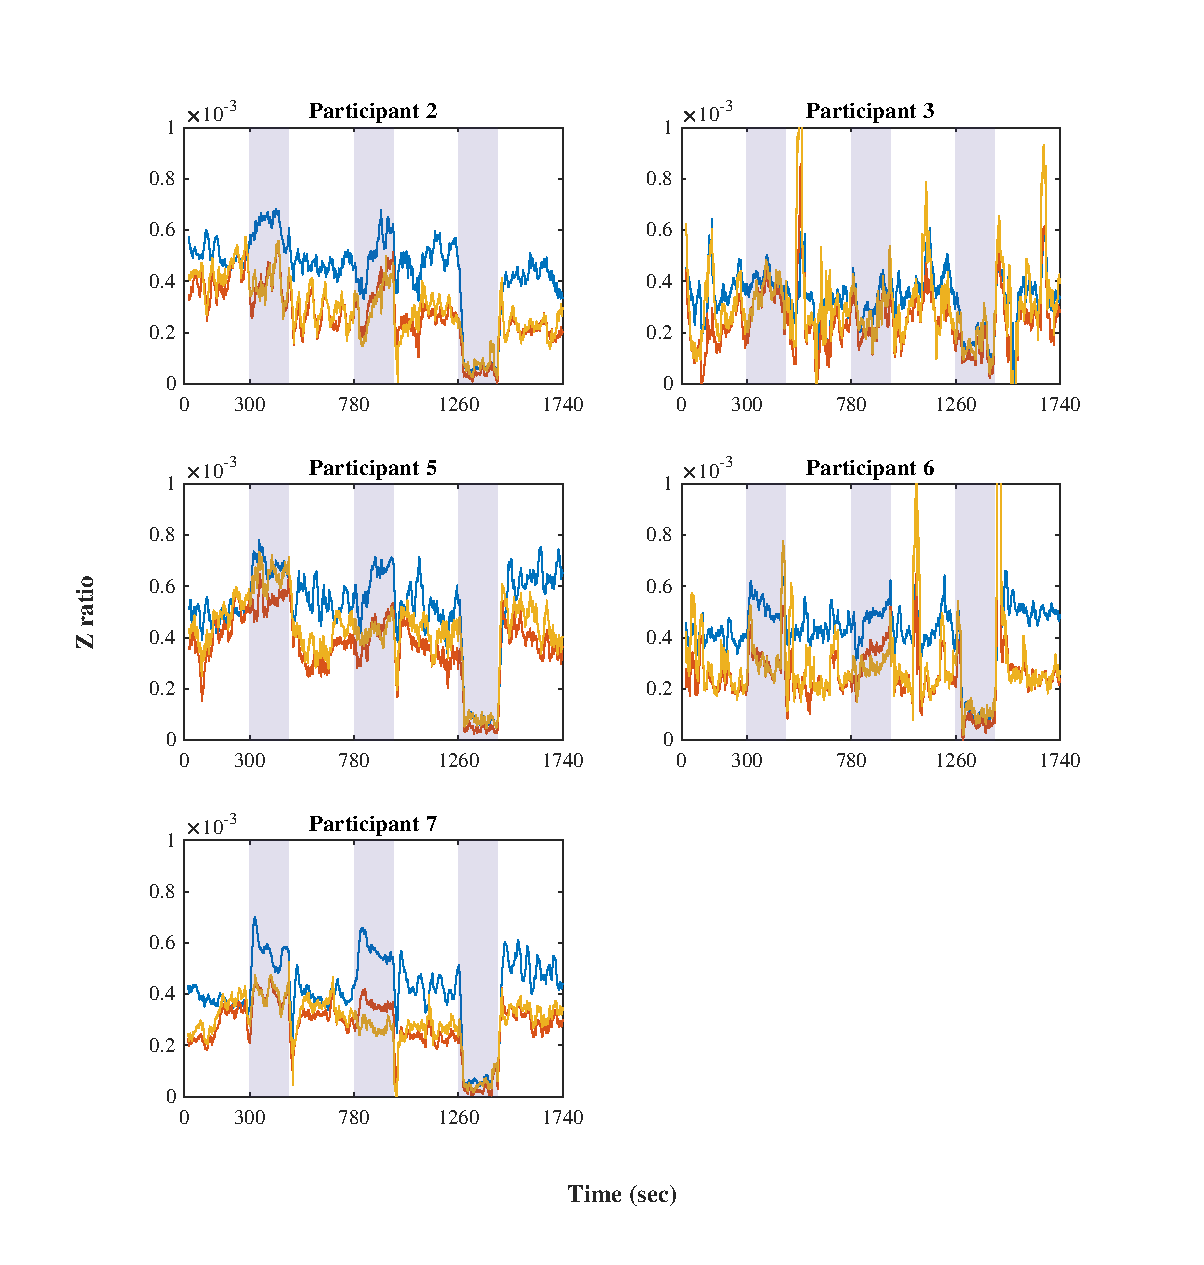
\includegraphics[width=1\textwidth,keepaspectratio]{figure1}    
 	\caption[Ratio of the plethysmography waveform over basal impedance during the experiment]{Measurement of the ratio between the plethysmography waveform over basal impedance during the whole experiment. The blue line represents the systolic peaks, the yellow line the dicrotic notch and the red line the diastolic peak.}
 	\label{fig:ratio Z}
 \end{figure}

Therefore, it is proposed a ratio indicator between the plethysmography waveform and the basal impedance as a method to differentiate between venous and arterial problems. For this method to work, it is necessary to identify the three points of the plethysmographic waveform, systolic peak, dicrotic notch and diastolic peak. The calculation of the ratio can be performed using the following equation.

\begin{align}
	\label{eq:ratio Z}
	i_Z = \frac{Z_{PG}}{Z_{BAS}}
\end{align}


This is a dimensionless index with three indicators referencing each point of the plethysmography waveform. This method was applied to the participants in the study, and the results were portrayed in figure \ref{fig:ratio Z}. As the graph shows, for most of the data, the systolic peak is over the other two signals. When a venous or partial arterial occlusion occurs (regions 2 and 4), there is an increment in the index. 

The dicrotic notch and the diastolic peak seem to change as a matching pair for most of the baseline signals where the dicrotic notch looks like being slightly lower than the diastolic peak. However, at the time of partial arterial blockage, the systolic index drops below the dicrotic notch index. This event is a clear differentiator between both types of flow restriction.

%********************************** % Third Section  *************************************
\section{Option to evaluate blood obstructions using iPG DC and AC waveforms}  %Section - 7.3 
\label{section discussion 3}
As it was described from the estimation of the blood from the impedance signal could not be a good indicator of circulatory disturbances in either the arterial or venous path. One reason for this, it is that mathematical expression describes there is a direct relation between the amplitude of the wave and the estimation of blood flow. However, when a mechanical constriction of the arm occurs in the venous or arterial circulation the amplitude of the waveform increases. Therefore, this increase in the $\Delta R$ will be calculated as an increase in blood flood which is not altogether correct. 

For this reason, it is proposed a method where it is possible to detect problems in the circulatory path by quantifying and analysing differences in the waveform of the impedance plethysmography signal shape. As it was described in the section \ref{section apa 1}, there are three reference points that can be used to describe an impedance plethysmography waveform. Normally, a non disturbed waveform is represented as systolic peak (point A) higher than the diastolic peak (point C) and the dicrotic notch point (point B) lower than those peaks. 

However, as it has been noticed when a venous occlusion occurs, there are changes in the waveform's shape that are distinguishable with each phenomena. The first event that can be noticed is that the systolic peak increases in size. It seems that these gain of size is due to the blood pooling in the veins. Venous occlusion experienced this effect as well as the partial arterial occlusion. However, it must be noticed that partial arterial blockage is also a type of venous occlusion where it restricts the blood flow coming into the forearm. Hence, it is expected to also show an rise in the systolic peak. 

Also, during the venous occlusion can be seen that most of the participants experienced an increase in the magnitude of the dicrotic notch and the diastolic peak. Consequently, it can be said that increase in the impedance plethysmography waveform may represent restriction in the venous circulation towards the forearm. 

Nonetheless, this is not the only indicator of a venous circulatory problem. Likewise, the basal impedance also varies during this kind of occlusion because of the increase of blood volume in the veins. As a result, the basal impedance also decreases in time. Which is also an indicator of circulatory problem. So, presenting these two values in one quantifying number could provide a better indicator of blood flow restriction. 

\begin{figure}[!htpb]
	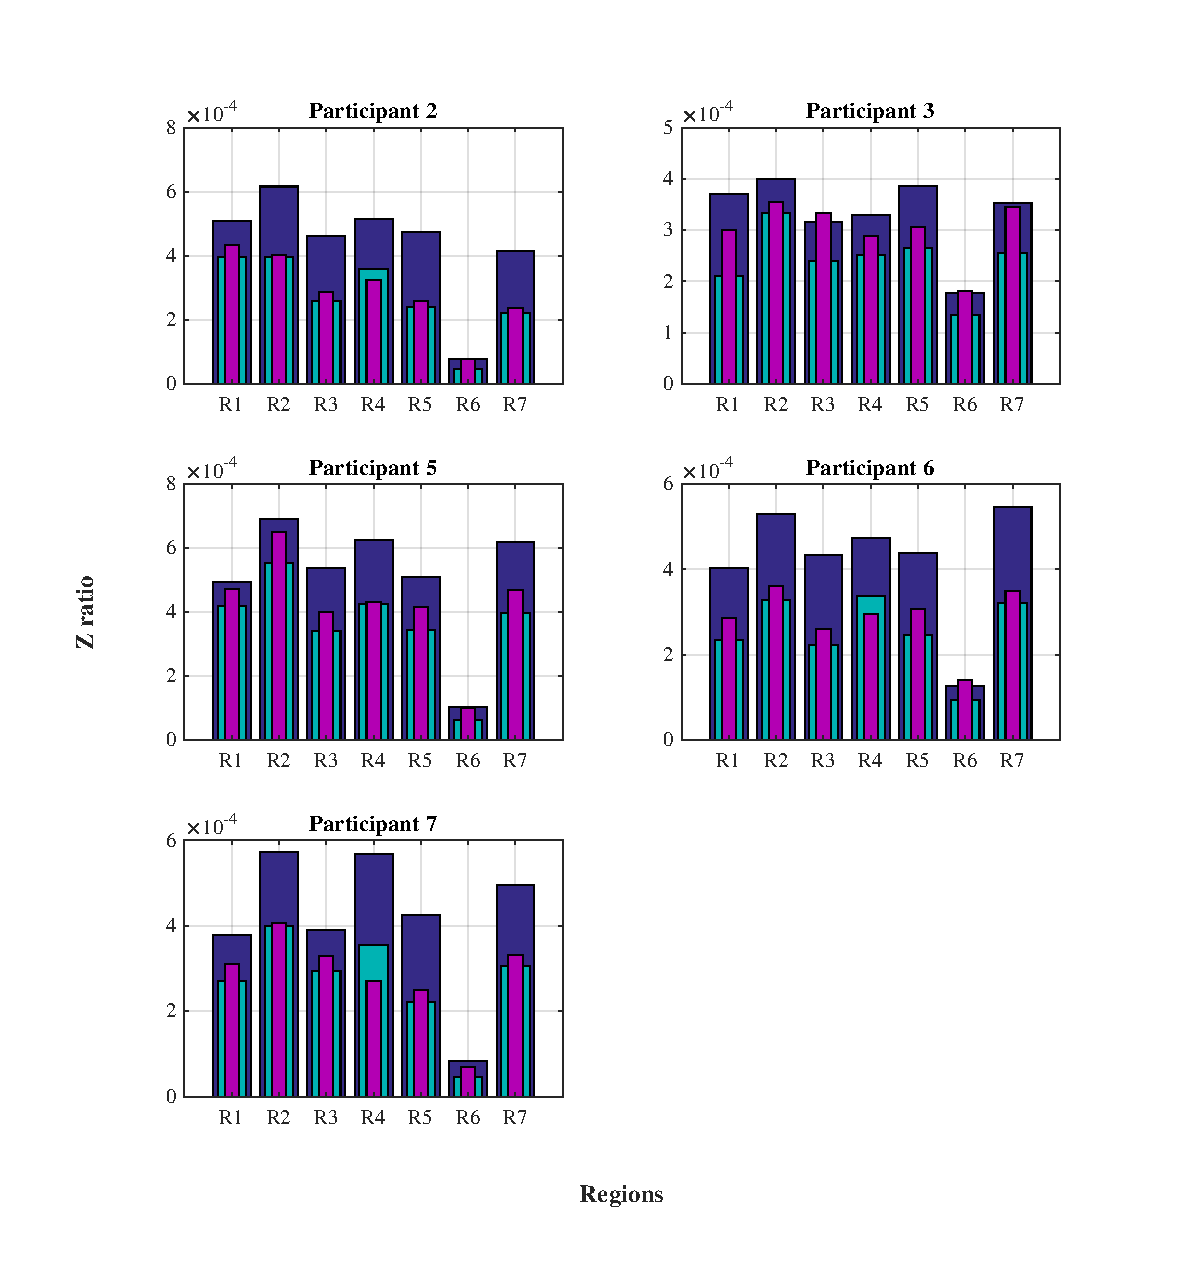
\includegraphics[width=1\textwidth,keepaspectratio]{figure2}    
	\caption[Bland and Altman plot of the relation between LDF and iPG]{Bland and Altman~\cite{bland1986statistical} plot of the relation between LDF and iPG. Data set corresponds to participants 2, 5, 6 and 7. The data has been normalised comparing the amplitude of both measurements. The different regions has been plotted with various colours and symbols to differentiate every event. The dotted line represents the perfect agreement, the dark line is the linear regression.}
	\label{fig:ration Z bar}
\end{figure}

\rvmynote{I have to double check the caption of this figure is not accurate}

\section{Future work}
The present work showed an initial prototype to measure iPG in an upper limb. There are improvements that can be done to the system from the hardware and software point of view. Furthermore, some experiments can be suggested to confirm if changes in the iPG waveform are caused by a body response or if there is a differentiator between arterial and venous components of the measurement. 

\subsection{Improvements of the iPG device}
The device had a good performance during all the tests performed. However, there are items of interest that could be implemented in future generations. From the design point of view, there is room to miniaturise the instrument. For this initial prototype, a modular approach was used. Nonetheless, designing an integrated PCB which could include the MCU on board as well as DAQ system will simplify the design considerably. Some challenges may arise for the design of the board. During the manufacturing of the PCB, it was found that combining digital with analogue channels increased the crosstalk between signals. Therefore, special care must be taken when designing a board of these characteristics. 

Complementary to this improvement, the device could accommodate a small set of batteries. This instrument included battery packs of \SI{12}{\volt} but if lower power banks were installed a better portability could be achieved. Furthermore, using a small current could be an option to use a smaller battery bank. However, additional challenges may arise. For instance, the impedance magnitude will get closer to the floor noise when using a  lower electrical current. Therefore, the noise will cover the signal of interest. 

Another improvement to the design will be the analysis of the phase of the signal. As most of the bioelectrical impedance devices, the instrument only measured the magnitude of the impedance. However, additional information about either volume or flow haemodynamics may lay under the phase shift data. Therefore, a channel dedicated to the phase could be an interesting add-on for future research. Nonetheless, there are quite a few challenges to achieve this. First, the contribution of the phase shift at the frequency used was about \SI{12}{\percent}. Therefore, the level of noise at that level can be quite challenging. Possibly, using a high frequency could be an option, but then the real part of the signal will be affected.

\subsection{Waveform analysis under different conditions}
The use of additional instruments provided information of changes in blood volume, arterial flow and micro-circulation. However, it could be of high interest to compare the iPG waveforms and NIRS method. The latter can provide data about tissue oxygenation, and within the basal impedance reading yields information about the amount of blood in the tissue. Therefore, it can be established how effective is the iPG to measure perfusion changes compared to an optic method.

The analysis of the waveforms showed differences when calculating the blood flow during venous and partial arterial occlusion. The results presented during the experimented suggests and increase of the blood flow which can only being explained by a vasodilation caused by a syncopal response. However, it could be recommended to perform cold tests to investigate if the narrowing of the vessels also display changes in the dicrotic notch point. 


